%-----------------------------------------------------------------------------
%
%               Template for sigplanconf LaTeX Class
%
% Name:         sigplanconf-template.tex
%
% Purpose:      A template for sigplanconf.cls, which is a LaTeX 2e class
%               file for SIGPLAN conference proceedings.
%
% Author:       Paul C. Anagnostopoulos
%               Windfall Software
%               978 371-2316
%               paul@windfall.com
%
% Created:      15 February 2005
%
%-----------------------------------------------------------------------------

\newif\ifieee
\ieeetrue
\newif\ifsubmit
\submittrue
% \submitfalse

%\documentclass[natbib,10pt,preprint]{sigplanconf}
\documentclass[10pt,conference]{IEEEtran}
%\documentclass[10pt,conference]{sigplanconf}

% The following \documentclass options may be useful:
%
% 10pt          To set in 10-point type instead of 9-point.
% 11pt          To set in 11-point type instead of 9-point.
% authoryear    To obtain author/year citation style instead of numeric.

\usepackage{amsmath}
\usepackage{graphicx}
\usepackage{fixltx2e}
\usepackage{fancyvrb}
\usepackage{subfigure}
\usepackage{hyphenat}
\usepackage{url}
%\usepackage[noadjust]{cite}

% squeeze more paper in - increase this value
\addtolength{\textwidth}{0.0in}

\begin{document}

\ifieee
\else
\conferenceinfo{Scala Days '11}{Stanford, CA} 
\copyrightyear{2011} 
\copyrightdata{[to be supplied]} 
\fi

%\titlebanner{Submitted to CGO '11 for confidential anonymous review} % These are ignored unless
%\preprintfooter{MAO - an Extensible Micro-Architectural Optimizer}   % 'preprint' option specified.

\title{Loop Recognition in C++/Java/Go/Scala}
%\subtitle{Subtitle Text, if any}

\ifsubmit 
\ifieee
\author{\IEEEauthorblockN{Robert~Hundt}
        \IEEEauthorblockA{
                          Google \\
                          1600 Amphitheatre Parkway \\
                          Mountain View, CA, 94043 \\
                          rhundt@google.com
                          }
       }

\else
\authorinfo{Robert Hundt}
           {Google\par
            1600 Amphitheatre Parkway\par
            Mountain View, CA, 94043
            }
           {rhundt@google.com}
\fi
\else
\authorinfo{}{}{}
\fi
\maketitle
\begin{abstract}
In this experience report we encode a well specified, compact
benchmark in four programming languages, namely C++, Java, Go, and
Scala.  The implementations each use the languages' idiomatic
container classes, looping constructs, and memory/object allocation
schemes. It does not attempt to exploit specific language and run-time
features to achieve maximum performance.  This approach allows an
almost fair comparison of language features, code complexity,
compilers and compile time, binary sizes, run-times, and memory
footprint.
 
While the benchmark itself is simple and compact, it employs many
language features, in particular, higher-level data structures (lists,
maps, lists and arrays of sets and lists), a few algorithms
(union/find, dfs / deep recursion, and loop recognition based on
Tarjan), iterations over collection types, some object oriented
features, and interesting memory allocation patterns.  We do not
explore any aspects of multi-threading, or higher level type
mechanisms, which vary greatly between the languages.

The benchmark points to very large differences in all examined
dimensions of the language implementations. After publication of the
benchmark internally at Google, several engineers produced highly
optimized versions of the benchmark. We describe many of the performed
optimizations, which were mostly targeting run-time performance and code
complexity. While this effort is an anecdotal comparison only,
the benchmark, and the subsequent tuning efforts, are indicative of
typical performance pain points in the respective languages.

\end{abstract}

\ifieee
\else
\category{D.3.4}{Processors}{Compilers}
\category{D.3.4}{Processors}{Optimization}

\terms
Performance

\keywords
Optimization, Performance
\fi

% Paper


\section{Introduction}

Disagreements about the utility of programming languages are
as old as programming itself. Today,
these ``language wars'' become increasingly heated, and less meaningful, as
more people are working with more languages on more platforms in settings of
greater variety, e.g., from mobile to datacenters.

In this paper, we contribute to the discussion by implementing a well
defined algorithm in four different languages, C++, Java, Go, and
Scala. In all implementations, we use the default, idiomatic data
structures in each language, as well as default type systems, memory
allocation schemes, and default iteration constructs. All four
implementations stay very close to the formal specification of the
algorithm and do not attempt any form of language specific
optimization or adaption.

The benchmark itself is simple and compact. Each implementation
contains some scaffold code, needed to construct test cases
allowing to benchmark the algorithm, and the implementation of the
algorithm itself.

The algorithm employs many language features, in particular,
higher-level data structures (lists, maps, lists and arrays of sets
and lists), a few algorithms (union/find, dfs / deep recursion, and
loop recognition based on Tarjan), iterations over collection types,
some object oriented features, and interesting memory allocation
patterns.  We do not explore any aspects of multi-threading, or higher
level type mechanisms, which vary greatly between the languages. We
also do not perform heavy numerical computation, as this omission
allows amplification of core characteristics of the language
implementations, specifically, memory utilization
patterns.

We believe that this approach highlights features and characteristics
of the languages and allows an almost fair comparison along the
dimensions of source code complexity, compilers and default libraries,
compile time,
binary sizes, run-times, and memory footprint. The differences along
these dimensions are surprisingly large.

After publication of the benchmark internally at Google, several
engineers produced highly optimized versions of the benchmark.  We
describe many of the performed optimizations, which were mostly
targeting run-time performance and code complexity. While this
evaluation is an anecdotal comparison only, the benchmark itself, as
well as the subsequent tuning efforts, point to typical performance
pain points in the respective languages.

The rest of this paper is organized as follows. We briefly introduce
the four languages in section \ref{contenders}.  We introduce the
algorithm and provide instructions on
how to find, build, and run it, in section \ref{algo}. 
We highlight core language properties in section
\ref{props}, as they are needed to understand the implementation and
the performance properties. We describe the benchmark and
methodology in section \ref{benchmark}, which also contains the
performance evaluation. We discuss subsequent language
specific tuning efforts in section \ref{tuning}, before we conclude.
 
 

\section{The contenders}
\label{contenders}

We describe the four languages by providing links to the  
the corresponding wikipedia entries and cite the respective first paragraphs
from wikipedia. 
Readers familiar with the languages can skip to the next section.

{\em C++} \cite{lang-cpp} is a statically typed,
free-form, multi-paradigm, compiled, general-purpose programming
language. It is regarded as a "middle-level" language, as it comprises
a combination of both high-level and low-level language features.
It was developed by Bjarne Stroustrup starting in 1979 at Bell Labs as
an enhancement to the C language and originally named C with
Classes. It was renamed C++ in 1983.


{\em Java} \cite{lang-java} is
a programming language originally developed by James Gosling at Sun
Microsystems (which is now a subsidiary of Oracle Corporation) and
released in 1995 as a core component of Sun Microsystems' Java
platform. The language derives much of its syntax from C and C++ but
has a simpler object model and fewer low-level facilities. Java
applications are typically compiled to byte-code (class file) that can
run on any Java Virtual Machine (JVM) regardless of computer
architecture. Java is a general-purpose, concurrent, class-based,
object-oriented language that is specifically designed to have as few
implementation dependencies as possible. It is intended to let
application developers "write once, run anywhere". Java is currently
one of the most popular programming languages in use, and is widely
used from application software to web applications.


{\em Go} \cite{lang-go} is a
compiled, garbage-collected, concurrent programming language developed
by Google Inc.  The initial design of Go was started in September 2007
by Robert Griesemer, Rob Pike, and Ken Thompson, building on previous
work related to the Inferno operating system. Go was officially
announced in November 2009, with implementations released for the
Linux and Mac OS X platforms. At the time of its launch, Go was not
considered to be ready for adoption in production environments. In May
2010, Rob Pike stated publicly that Go is being used "for real stuff"
at Google.

{\em Scala} \cite{lang-scala}
is a multi-paradigm programming language designed to integrate
features of object-oriented programming and functional
programming. The name Scala stands for "scalable language", signifying
that it is designed to grow with the demands of its users.

Core properties of these languages are:

\begin{itemize}

\item C++ and Go are statically compiled, both Java and Scala run on
  the JVM, which means code is compiled to Java Byte Code, which is 
  interpreted and/or compiled dynamically.

\item All languages but C++ are garbage collected, where Scala and
  Java share the same garbage collector.

\item C++ has pointers, Java and Scala has no pointers, and Go makes
  limited use of pointers.

\item C++ and Java require statements being terminated with a
  ';'. Both Scala and Go don't require that. Go's algorithm enforces
  certain line breaks, and with that a certain coding style. While Go's
  and Scala's algorithm for semicolon inference are 
  different, both algorithms are intuitive and powerful.

\item C++, Java, and Scala don't enforce specific coding styles. As a
  result, there are many of them, and many larger programs have many
  pieces written in different styles. The C++ code is written
  following Google's style guides, the Java and Scala code (are trying
  to) follow the official Java style guide. Go's programming style is
  strictly enforced -- a Go program is only valid if it comes
  unmodified out of the automatic formatter {\tt gofmt}.

\item Go and Scala have powerful type inference, making explicit type
  declarations very rare. In C++ and Java everything needs to be
  declared explicitly.

\item C++, Java, and Go, are object-oriented. Scala is object-oriented
  and functional, with fluid boundaries.

\end{itemize}


\section{The Algorithm}
\label{algo}

The benchmark is an implementation of the loop recognition algorithm
described in "Nesting of reducible and irreducible loops", by Havlak,
Rice University, 1997, \cite{havlak}.  The algorithm itself is an
extension to the algorithm described R.E. Tarjan, 1974, Testing flow
graph reducibility \cite{Tarjan:1983}. 
It further employs the Union/Find algorithm
described in "Union/Find Algorithm", Tarjan, R.E., 1983, Data
Structures and Network Algorithms \cite{Tarjan:1973}.

The algorithm formulation in Figure \ref{algofig}, as well as the
various implementations, follow the nomenclature using variable names
from the algorithm in Havlak's paper, which in turn follows the Tarjan
paper.

\begin{figure}
%\includegraphics[width=85mm]{algo2cropped.pdf}
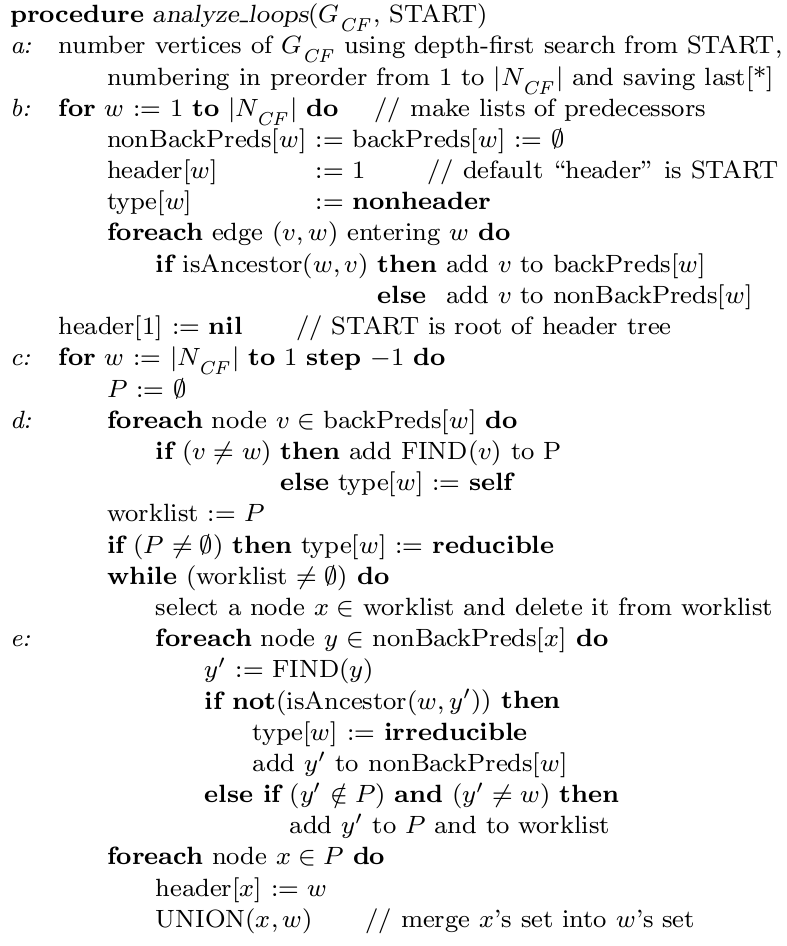
\includegraphics[width=85mm]{havlaklarge.png}
\caption{Finding headers of reducible and irreducible loops. This 
    presentation is a literal copy from the original paper \cite{havlak}}
\label{algofig}
\end{figure}

The full benchmark sources are available as open-source, hosted
by Google code at {\tt http://code.google.com/p/} in the project
{\tt multi-language-bench}.
The source files contain the main algorithm
implementation, as well as dummy classes to
construct a control flow graph (CFG), a loop structure graph (LSG),
and a driver program for benchmarking (e.g., {\tt LoopTesterApp.cc}).

As discussed, after an internal version of this document was published
at Google, several engineers created optimized versions of the
benchmark. We feel that the optimization techniques applied for each
language were interesting and indicative of the issues
performance engineers are facing in their every day experience.  The
optimized versions are kept in the {\em Pro} versions of the
benchmarks. At time of this writing, the {\tt cpp\_pro} version
depended strongly on Google specific code and could not be open-sourced.
All directories in Figure \ref{sourcedirs} are found in the
{\tt havlak} directory.

Each directory contains a {\tt Makefile} and supports three
methods of invocation:

\begin{footnotesize}
\begin{verbatim}
  make       # build benchmark
  make run   # run benchmark
  make clean # clean up build artifacts
\end{verbatim}
\end{footnotesize}

Path names to compilers and libraries can be overridden
on the command lines. Readers interested in running the benchmarks
are encouraged to study the very short {\tt Makefiles} for 
more details.

\begin{figure}
\begin{tabular}{ll}
{\tt\small src           }  & README file and auxiliary scripts  \\
{\tt\small src/cpp       }  & C++ version \\
{\tt\small src/cpp\_pro  }  & Improved by Doug Rhode \\
{\tt\small src/scala     }  & Scala version \\
{\tt\small src/scala\_pro}  & Improved by Daniel Mahler \\
{\tt\small src/go        }  & Go version \\
{\tt\small src/go\_pro   }  & Improved by Ian Taylor \\
{\tt\small src/java      }  & Java version \\
{\tt\small src/java\_pro }  & Improved by Jeremy Manson \\
{\tt\small src/python    }  & Python version (not discussed here) \\
\end{tabular}
\caption{Benchmark source organization (at the time of this writing,
the cpp\_pro version could not yet be open-sourced)}
\label{sourcedirs}
\end{figure}


\section{Implementation Notes}
\label{props}

This section highlights a few core language properties, as necessary to 
understanding the benchmark sources and performance characteristics. 
Readers familiar with the languages can safely skip to the next section.

\subsection{Data Structures}

The key data structures for the implementation of the algorithm are
shown in Figure \ref{datastructs}. Please note again that we are
strictly following the algorithm's notation. We do not seek to apply
any manual data structure optimization at this point. We use the
non object-oriented, quirky notation of the paper, and we only
use the languages' default containers.

\begin{figure}
\begin{tabular}{ll}
{\tt\small non\_back\_preds} & an array of sets of int's  \\
{\tt\small back\_preds} & an array of lists of int's  \\
{\tt\small header} & an array of int's \\
{\tt\small type  } & an array of char's  \\
{\tt\small last  } & an array of int's \\
{\tt\small nodes } & an array of union/find nodes \\
{\tt\small number} & a map from basic blocks to int's \\
\end{tabular}
\caption{Key benchmark data structures, modeled after the original paper}
\label{datastructs}
\end{figure}

\subsubsection{C++} 
With the standard library and templates, these data structures are defined the following way in C++ using stack local variables:

\begin{footnotesize}
\begin{verbatim}
  typedef std::vector<UnionFindNode>  NodeVector;
  typedef std::map<BasicBlock*, int>  BasicBlockMap;
  typedef std::list<int>              IntList;
  typedef std::set<int>               IntSet;
  typedef std::list<UnionFindNode*>   NodeList;
  typedef std::vector<IntList>        IntListVector;
  typedef std::vector<IntSet>         IntSetVector;
  typedef std::vector<int>            IntVector;
  typedef std::vector<char>           CharVector;
[...]
    IntSetVector       non_back_preds(size);
    IntListVector      back_preds(size);
    IntVector          header(size);
    CharVector         type(size);
    IntVector          last(size);
    NodeVector         nodes(size);
    BasicBlockMap      number;
\end{verbatim}
\end{footnotesize}

The size of these data structures is known at run-time and the {\tt
  std::} collections allow pre-allocations at those sizes, except for
the map type.

\subsubsection{Java} 

Java does not allow arrays of generic types. However, lists are
index-able, so this code is permissible:

\begin{footnotesize}
\begin{verbatim}
List<Set<Integer>>  nonBackPreds = 
               new ArrayList<Set<Integer>>();
List<List<Integer>> backPreds = 
               new ArrayList<List<Integer>>();
int[]               header = new int[size];
BasicBlockClass[]   type = 
               new BasicBlockClass[size];
int[]               last = new int[size];
UnionFindNode[]     nodes = new UnionFindNode[size];
Map<BasicBlock, Integer> number = 
               new HashMap<BasicBlock, Integer>();
\end{verbatim}
\end{footnotesize}

However, this appeared to incur tremendous GC overhead. In order to
alleviate this problem we slightly rewrite the code, which reduced GC
overhead modestly.

\begin{footnotesize}
\begin{verbatim}
    nonBackPreds.clear();
    backPreds.clear();
    number.clear();
    if (size > maxSize) {
      header = new int[size];
      type = new BasicBlockClass[size];
      last = new int[size];
      nodes = new UnionFindNode[size];
      maxSize = size;
    }
\end{verbatim}
\end{footnotesize}

Constructors still need to be called:

\begin{footnotesize}
\begin{verbatim}
    for (int i = 0; i < size; ++i) {
      nonBackPreds.add(new HashSet<Integer>());
      backPreds.add(new ArrayList<Integer>());
      nodes[i] = new UnionFindNode();
    }
\end{verbatim}
\end{footnotesize}

To reference an element of the {\tt ArrayLists},  the {\tt get/set}
methods are used, like this:

\begin{footnotesize}
\begin{verbatim}
   if (isAncestor(w, v, last)) {
            backPreds.get(w).add(v);
          } else {
            nonBackPreds.get(w).add(v);
          }
\end{verbatim}
\end{footnotesize}


\subsubsection{Scala}

Scala allows arrays of generics, as an array is just a language
extension, and not a built-in concept. Constructors still need to be
called:

\begin{footnotesize}
\begin{verbatim}
var nonBackPreds = new Array[Set[Int]](size)
var backPreds    = new Array[List[Int]](size)
var header       = new Array[Int](size)
var types        = 
           new Array[BasicBlockClass.Value](size)
var last         = new Array[Int](size)
var nodes        = new Array[UnionFindNode](size)
var number       = 
   scala.collection.mutable.Map[BasicBlock, Int]()

for (i <- 0 until size) {
    nonBackPreds(i) = Set[Int]()
    backPreds(i)    = List[Int]()
    nodes(i)        = new UnionFindNode()
}
\end{verbatim}
\end{footnotesize}

With clever use of parenthesis (and invocation of {\tt apply()}
accesses become more canonical, e.g.:


\begin{footnotesize}
\begin{verbatim}
     if (isAncestor(w, v, last)) {
         backPreds(w) = v :: backPreds(w)
     } else {
         nonBackPreds(w) += v
     }
\end{verbatim}
\end{footnotesize}

\subsubsection{Go}

This language offers the {\tt make} keyword in addition to the {\tt
  new} keyword.  {\tt Make} takes away the pain of the explicit
constructor calls. A map is a built-in type, and has a special syntax,
as can be seen in the 1st line below. There is no {\tt set} type, so in
order to get the same effect, one can use a map to {\tt bool}. While
maps are built-in, lists are not, and as a result accessors and
iterators become non-canonical.

\begin{footnotesize}
\begin{verbatim}
 nonBackPreds := make([]map[int]bool, size)
 backPreds := make([]list.List, size)
 number := make(map[*cfg.BasicBlock]int)
 header := make([]int, size, size)
 types := make([]int, size, size)
 last := make([]int, size, size)
 nodes := make([]*UnionFindNode, size, size)

 for i := 0; i < size; i++ {
 nodes[i] = new(UnionFindNode)
 }
\end{verbatim}
\end{footnotesize}




%------------------------------------------------------------------------------


\subsection{Enumerations}

To enumerate the various kinds of loops an
enumeration type is used. The following subsections show
what the languages offer to express compile time constants.

\subsubsection{C++}
In C++ a regular {\tt enum} type can be used

\begin{footnotesize}
\begin{verbatim}
  enum BasicBlockClass {
    BB_TOP,          // uninitialized
    BB_NONHEADER,    // a regular BB
    BB_REDUCIBLE,    // reducible loop
    BB_SELF,         // single BB loop
    BB_IRREDUCIBLE,  // irreducible loop
    BB_DEAD,         // a dead BB
    BB_LAST          // Sentinel
  };
\end{verbatim}
\end{footnotesize}

\subsubsection{Java}

Java has quite flexible support for enumeration types. Specifically,
enum members can have constructor parameters, and enums also offer
iteration via {\tt values()}. Since the requirements for this
specific benchmark are trivial, the code
looks similarly simple:

\begin{footnotesize}
\begin{verbatim}
  public enum BasicBlockClass {
    BB_TOP,          // uninitialized
    BB_NONHEADER,    // a regular BB
    BB_REDUCIBLE,    // reducible loop
    BB_SELF,         // single BB loop
    BB_IRREDUCIBLE,  // irreducible loop
    BB_DEAD,         // a dead BB
    BB_LAST          // Sentinel
  }
\end{verbatim}
\end{footnotesize}


\subsubsection{Scala}

In Scala, enumerations become a static instance of a type derived from
{\tt Enumeration}. The syntax below calls and increments {\tt Value()}
on every invocation (parameterless function calls don't need
parenthesis in Scala). Note that, in this regard, enums are not a
language feature, but an implementation of the method {\tt
  Enumeration.Value()}.  {\tt Value} also offers the ability to
specify parameter values, similar to the Java enums with constructors.

\begin{footnotesize}
\begin{verbatim}
  class BasicBlockClass extends Enumeration {
  }
  object BasicBlockClass extends Enumeration {
    val BB_TOP,      // uninitialized
    BB_NONHEADER,    // a regular BB
    BB_REDUCIBLE,    // reducible loop
    BB_SELF,         // single BB loop
    BB_IRREDUCIBLE,  // irreducible loop
    BB_DEAD,         // a dead BB
    BB_LAST = Value  // Sentinel
  }
\end{verbatim}
\end{footnotesize}

\subsubsection{Go}

Go has the concept of an {\tt iota} and initialization expression. For
every member of an enumeration (constants defined within a {\tt const}
block), the right hand side expression will be executed in full, with
{\tt iota} being incremented on every invocation. {\tt iota} is being reset on
encountering the {\tt const} keyword. This makes for flexible initialization
sequences, which are not shown, as the use case is trivial. Note that
because of Go's powerful line-breaking, not even a comma is needed. Furthermore,
because of Go's symbol exporting rules, the first characters of the
constants are held lower case (see comments on symbol binding later).

\begin{footnotesize}
\begin{verbatim}
const (
 _             = iota // Go has the iota concept
 bbTop                // uninitialized
 bbNonHeader          // a regular BB
 bbReducible          // reducible loop
 bbSelf               // single BB loop
 bbIrreducible        // irreducible loop
 bbDead               // a dead BB
 bbLast               // sentinel
)
\end{verbatim}
\end{footnotesize}



%------------------------------------------------------------------------

\subsection{Iterating over Data Structures}

\subsubsection{C++}

C++ has no "special" built-in syntactical support for iterating over
collections (e.g., the upcoming range-based for-loops in
C++0x). However, it does offer templates, and all basic data
structures are now available in the standard library. Since the
language support is minimal, to iterate, e.g., over a list of
non-backedges, one has to write:

\begin{footnotesize}
\begin{verbatim}
// Step d:
IntList::iterator back_pred_iter = 
           back_preds[w].begin();
IntList::iterator back_pred_end  = 
           back_preds[w].end();
for (; back_pred_iter != back_pred_end; 
       back_pred_iter++) {
     int v = *back_pred_iter;
\end{verbatim}
\end{footnotesize}

To iterate over all members of a map:

\begin{footnotesize}
\begin{verbatim}
for (MaoCFG::NodeMap::iterator bb_iter =
     CFG_->GetBasicBlocks()->begin();
    bb_iter != CFG_->GetBasicBlocks()->end(); 
      ++bb_iter) {
    number[(*bb_iter).second] = kUnvisited;
}
\end{verbatim}
\end{footnotesize}

\subsubsection{Java}

Java is aware of the base interfaces supported by collection types and
 offers an elegant language extension for easier iteration. In a
 sense, there is "secret" handshake between the run time libraries and
 the Java compiler. The same snippets from above look like the following in
 Java:

\begin{footnotesize}
\begin{verbatim}
      // Step d:
      for (int v : backPreds.get(w)) {
\end{verbatim}
\end{footnotesize}

and for the map:

\begin{footnotesize}
\begin{verbatim}
    for (BasicBlock bbIter : 
           cfg.getBasicBlocks().values()) {
      number.put(bbIter, UNVISITED);
\end{verbatim}
\end{footnotesize}

\subsubsection{Scala}

Scala offers similar convenience for iterating over lists:

\begin{footnotesize}
\begin{verbatim}
    // Step d:
    for (v <- backPreds(w)) {
\end{verbatim}
\end{footnotesize}

and for maps iterations:

\begin{footnotesize}
\begin{verbatim}
    for ((key, value) <- cfg.basicBlockMap) {
      number(value) = UNVISITED
    }
\end{verbatim}
\end{footnotesize}

These "for-comprehensions" are very powerful. Under the hood, the
compiler front-end builds closures and transforms the code into
combinations of calls to {\tt map(), flatmap{}, filter()}, and {\tt
  foreach()}. Loop nests and conditions can be expressed
elegantly. Each type implementing the base interfaces can be used in
for-comprehensions. This can be used for elegant language
extensions. On the downside - since closures are being built, there is
performance overhead. The compiler transforms the for-comprehensions
and therefore there is also has a "secret" hand-shake between
libraries and compiler. More details on Scala for-comprehensions can
be found in Section 6.19 of the Scala Language Specification
\cite{Scala-ref}.

Note that in the example, the tuple on the left side of the
arrow is not a built-in language
construct, but cleverly written code to mimic and implement tuples.

\subsubsection{Go}

Lists are not built-in, and they are also not type-safe. As a result,
iterations are more traditional and require explicit casting. For
example:

\begin{footnotesize}
\begin{verbatim}
// Step d:
for ll := backPreds[w].Front(); ll != nil; 
    ll = ll.Next() {
       v := ll.Value.(int)
\end{verbatim}
\end{footnotesize}

Since maps are built-in, there is special range keyword and the language allows returning tuples:

\begin{footnotesize}
\begin{verbatim}
for i, bb := range cfgraph.BasicBlocks() {
       number[bb] = unvisited
\end{verbatim}
\end{footnotesize}

Note that lists are inefficient in Go (see performance and memory
footprint below). The GO Pro version replaces most lists with array
slices, yielding significant performance gains (~25\%),
faster compile times, and more
elegant code.  We denote removed lines with {\tt -} and the replacement
lines with {\tt +}, similarly to the output of modern {\tt diff} tools.
For example, the LSG data structure changes:

\begin{footnotesize}
\begin{verbatim}
type LSG struct {
 	root  *SimpleLoop
-       loops list.List
+       loops []*SimpleLoop
 }
\end{verbatim}
\end{footnotesize}

and references in {\tt FindLoops()} change accordingly:

\begin{footnotesize}
\begin{verbatim}
  - backPreds := make([]list.List, size)
  + backPreds := make([][]int, size)
\end{verbatim}
\end{footnotesize}

and

\begin{footnotesize}
\begin{verbatim}
- for ll := nodeW.InEdges().Front(); ll != nil; 
-     ll = ll.Next() {
-       nodeV := ll.Value.(*cfg.BasicBlock)

+ for _, nodeV := range nodeW.InEdges {
\end{verbatim}
\end{footnotesize}

Note that both Go and Scala use {\tt \_} as a placeholder.

\subsection{Type Inference}

C++ and Java require explicit type declarations.
Both Go and Scala have powerful type inference, which means that types
rarely need to be declared explicitly.

\subsubsection{Scala}

Because of Scala functional bias, variables or values must be declared
as such. However, types are inferred. For example:

\begin{footnotesize}
\begin{verbatim}
    var lastid = current
\end{verbatim}
\end{footnotesize}

\subsubsection{Go}

To declare and define a variable lastid and assign it the value from
an existing variable current, Go has a special assignment operator :=

\begin{footnotesize}
\begin{verbatim}
        lastid := current
\end{verbatim}
\end{footnotesize}

\subsection{Symbol Binding}

The languages offer different mechanism to control symbol bindings:

\subsubsection{C++}

C++ relies on the {\tt static} and {\tt external} keywords to specify symbol
bindings.

\subsubsection{Java}

Java uses packages and the {\tt public}
 keyword to control symbol binding.

\subsubsection{Scala}

Scala uses similar mechanism as Java, but there are differences in the
package name specification, which make things a bit more concise and
convenient. Details are online at \cite{scala-package-1} 
and \cite{scala-package-2}.

\subsubsection{Go}
Go uses a simple trick to control symbol binding. If a symbol's first
character is uppercase - it's being exported. 


\subsection{Member Functions}

\subsubsection{C++}

Google's coding style guidelines require that class members be
accessed through accessor functions. For C++, simple accessor
functions come with no performance penalty, as they are
inlined. Constructors are explicitly defined. For example, for
the {\tt BasicBlockEdge} class in the benchmarks, the code looks like the
following:

\begin{footnotesize}
\begin{verbatim}
class BasicBlockEdge {
 public:
  inline BasicBlockEdge(MaoCFG *cfg, 
                        int     from, 
                        int to);

  BasicBlock *GetSrc() { return from_; }
  BasicBlock *GetDst() { return to_; }

 private:
  BasicBlock *from_, *to_;
};
[...]
inline
BasicBlockEdge::BasicBlockEdge(MaoCFG  *cfg,
                               int      from_name,
                               int      to_name) {
  from_ = cfg->CreateNode(from_name);
  to_ = cfg->CreateNode(to_name);

  from_->AddOutEdge(to_);
  to_->AddInEdge(from_);

  cfg->AddEdge(this);
}
\end{verbatim}
\end{footnotesize}


\subsubsection{Java}

Java follows the same ideas, and the resulting code looks similar:

\begin{footnotesize}
\begin{verbatim}
public class BasicBlockEdge {
  public BasicBlockEdge(CFG cfg, 
                        int fromName, 
                        int toName) {
    from = cfg.createNode(fromName);
    to   = cfg.createNode(toName);

    from.addOutEdge(to);
    to.addInEdge(from);

    cfg.addEdge(this);
  }

  public  BasicBlock getSrc() { return from; }
  public  BasicBlock getDst() { return to; }

  private BasicBlock from, to;
};
\end{verbatim}
\end{footnotesize}

\subsubsection{Scala}

The same code can be expressed in a very compact fashion in Scala. The
class declaration allows parameters, which become instance variables
for every object. Constructor code can be placed directly into the
class definition. The variables {\tt from} and {\tt to} become accessible for users of
this class via automatically generated getter functions. Since
parameterless functions don't require parenthesis, such accessor
functions can always be rewritten later, and no software engineering
discipline is lost. Scala also produces setter functions,
which are named like the variables with an appended underscore. E.g.,
this code can use {\tt from\_(int)} and {\tt to\_(int)}
 without having to declare
them. The last computed value is the return value of a function,
saving on return statements (not applicable in this example)

\begin{footnotesize}
\begin{verbatim}
class BasicBlockEdge(cfg      : CFG, 
                     fromName : Int, 
                     toName   : Int) {
  var from : BasicBlock = cfg.createNode(fromName)
  var to   : BasicBlock = cfg.createNode(toName)
  
  from.addOutEdge(to)
  to.addInEdge(from)

  cfg.addEdge(this)
}
\end{verbatim}
\end{footnotesize}

\subsubsection{Go}

Go handles types in a different way. It allows declaration of types
and then the definition of member functions as traits to types. The
resulting code would look like this:

\begin{footnotesize}
\begin{verbatim}
 type BasicBlockEdge struct {
        to   *BasicBlock
        from *BasicBlock
 }

 func (edge *BasicBlockEdge) Dst() *BasicBlock {
        return edge.to
 }

 func (edge *BasicBlockEdge) Src() *BasicBlock {
         return edge.from
 }

 func NewBasicBlockEdge(cfg *CFG, from int, to int)
          *BasicBlockEdge {
       self := new(BasicBlockEdge)
       self.to = cfg.CreateNode(to)
       self.from = cfg.CreateNode(from)

       self.from.AddOutEdge(self.to)
       self.to.AddInEdge(self.from)

       return self
 }
\end{verbatim}
\end{footnotesize}

However, the 6g compiler does not inline functions and the resulting
code would perform quite poorly. Go also has the convention of
accessing members directly, without getter/setter
functions. Therefore, in the Go Pro version, the code is becoming a
lot more compact:

\begin{footnotesize}
\begin{verbatim}
 type BasicBlockEdge struct {
        Dst *BasicBlock
        Src *BasicBlock
 }
 
 func NewBasicBlockEdge(cfg *CFG, from int, to int) 
           *BasicBlockEdge {
        self := new(BasicBlockEdge)
        self.Dst = cfg.CreateNode(to)
        self.Src = cfg.CreateNode(from)

        self.Src.AddOutEdge(self.Dst)
        self.Dst.AddInEdge(self.Src)
 
        return self
 }
\end{verbatim}
\end{footnotesize}

\section{Performance Analysis}
\label{benchmark}

The benchmark consists of a driver for the loop recognition
functionality. This driver constructs a very simple control flow
graph, a diamond of 4 nodes with a backedge from the bottom to the
top node, and performs loop recognition on it for 15.000 times. 
The purpose is to force Java/Scala compilation, so that the benchmark 
itself can be measured on compiled code. 

Then the driver constructs a
large control flow graph containing 4-deep loop nests with a total of
76000 loops. It performs loop recognition on this graph for 50
times. The driver codes for all languages are identical.

As a result of this benchmark design, the Scala and Java measurements
contain a small fraction of interpreter time. However, this fraction
is very small and run-time results presented later should be
taken as ``order of magnitude'' statements only.

The benchmarking itself was done in a simple and fairly 
un-scientific fashion. The benchmarks were run 3 times and
the median values are reported. 
All of the experiments are done on an older Pentium IV workstation.
Run-times were measured using wall-clock time.
We analyze the benchmarks along the dimensions code size, compile time, binary
size, memory footprint, and run-time.

\subsection{Code Size}

The benchmark implementations contain similar comments in all codes,
with a few minor exceptions. Therefore, to compare code size, a simple
Linux {\tt wc} is performed on the benchmarking code and the main algorithm
code together, counting lines. The results are shown in Figure \ref{codesize}.
Code is an important factor in
program comprehension. Studies have shown that the average time to
recognize a token in code is a constant for individual programmers. As
a result, less tokens means goodness. Note that the Scala and Go
versions are significantly more compact than the verbose C++ and Java versions.

\begin{figure}
\begin{tabular}{|l|r|r|} \hline
 Benchmark	&wc -l	& Factor  \\ \hline\hline
 C++ Dbg/Opt	&850    & 1.3x	  \\ \hline
 Java 	        &1068	& 1.6x	  \\ \hline
 Java Pro       &1240	& 1.9x	  \\ \hline
 Scala	        &658	& 1.0x	  \\ \hline
 Scala Pro      &297	& 0.5x	  \\ \hline
 Go	        &902	& 1.4x	  \\ \hline
 Go Pro	        &786	& 1.2x	  \\ \hline
\end{tabular}
\caption{Code Size in $[$Lines of Code$]$, normalized to the Scala version}
\label{codesize}
\end{figure}

\subsection{Compile Times}

In Figure \ref{compiletime} we compare the static compile times for
the various languages. Note that Java/Scala only compile to
Java Byte Code. For Scala, the {\tt scalac} compiler is evaluated,
as well as the memory resident {\tt fsc} compiler, which avoids
re-loading of the compiler on every invocation. This benchmark
is very small in terms of lines of code, and unsurprisingly,
{\tt fsc} is about 3-4x faster than {\tt scalac}.

\begin{figure}
\begin{tabular}{|l|r|r|} \hline
 Benchmark    & Compile Time       & Factor \\ \hline\hline
 C++ Dbg      &      3.9           &  6.5x \\ \hline
 C++ Opt      &      3.0           &  5.0x \\ \hline
 Java         &      3.1           &  5.2x \\ \hline
 Java Pro     &      3.0           &  5.0x \\ \hline
 Scala scalac &     13.9           & 23.1x \\ \hline
 Scala fsc    &      3.8           &  6.3x \\ \hline
 Scala Pro scalac & 11.3           & 18.8x \\ \hline
 Scala Pro fsc    &  3.5           &  5.8x \\ \hline
 Go           &      1.2           &  2.0x \\ \hline
 Go Pro       &      0.6           &  1.0x \\ \hline
\end{tabular}
\caption{Compilation Times in $[$Secs$]$, normalized to the Go Pro version}
\label{compiletime}
\end{figure}


\subsection{Binary Sizes}

In Figure \ref{binsize} we compare the statically compiled binary
sizes, which may contain debug information, and JAR file sizes. Since
much of the run-time is not contained in Java JAR files, they are
expected to be much smaller in size and used as baseline.  It should
also be noted that for large binaries, plain binary size matters a
lot, as in distributed build systems, the generated binaries need to
be transferred from the build machines, which can be bandwidth limited and
slow.

\begin{figure}
\begin{tabular}{|l|r|r|} \hline
 Benchmark   & Binary or Jar [Byte] & Factor \\ \hline\hline
 C++ Dbg     &    592892           &   45x \\ \hline
 C++ Opt     &     41507           &  3.1x \\ \hline
 Java        &     13215           &  1.0x \\ \hline
 Java Pro    &     21047           &  1.6x \\ \hline
 Scala       &     48183           &  3.6x \\ \hline
 Scala Pro   &     36863           &  2.8x \\ \hline
 Go          &   1249101           &   94x \\ \hline
 Go Pro      &   1212100           &   92x \\ \hline
\end{tabular}
\caption{Binary and JAR File Sizes in $[$Byte$]$, normalized to the Java version}
\label{binsize}
\end{figure}


\subsection{Memory Footprint}

To estimate memory footprint, the benchmarks were run alongside
the Unix {\tt top} utility and memory values were manually
read out in the middle of the benchmark run.
The numbers are fairly stable across the benchmark
run-time. The first number in the table below 
represents potentially pre-allocated, but un-touched
virtual memory. The second number (Real) represents real memory used.

\begin{figure}
\begin{tabular}{|l|r|r|r|r|} \hline
 Benchmark	& Virt &Real &   Factor Virt  & Factor Real \\ \hline\hline
 C++ Opt	& 184m &163m & 	 1.0	      & 1.0 \\ \hline
 C++ Dbg	& 474m &452m & 	 2.6-3.0      & 2.8 \\ \hline
 Java	        &1109m &617m & 	 6.0	      & 3.7 \\ \hline
 Scala          &1111m &293m &   6.0	      & 1.8 \\ \hline
 Go	        &16.2g &501m & 	 90	      & 3.1 \\ \hline
\end{tabular}
\caption{Memory Footprint, normalized to the C++ version}
\label{codesize}
\end{figure}

\subsection{Run-time Measurements}

It should be noted that this benchmark is designed to amplify language
implementations' negative properties. There is lots of memory
traversal, so minimal footprint is beneficial. There is recursion, so
small stack frames are beneficial. There are lots of array accesses,
so array bounds checking will be negative. There are many objects
created and destroyed - this could be good or bad for the garbage
collector. As shown, GC settings have huge impact on
performance. There are many pointers used and null-pointer checking
could be an issue. For Go, some key data structures are part of the
language, others are not. The results are summarized in Figure \ref{runtime}.

\begin{figure}
\begin{tabular}{|l|r|r|} \hline
 Benchmark   & Time [sec] &	 Factor  \\ \hline\hline
 C++ Opt	& 23 	  & 1.0x \\ \hline
 C++ Dbg	&197 	  & 8.6x \\ \hline
 Java 64-bit	& 134 	  & 5.8x \\ \hline
 Java 32-bit	& 290	  &12.6x \\ \hline
 Java 32-bit GC* & 106	  &4.6x \\ \hline
 Java 32-bit SPEC GC & 89 &	 3.7x \\ \hline
 Scala 	             & 82 &	 3.6x \\ \hline
 Scala low-level*    & 67 &	 2.9x \\ \hline
 Scala low-level GC* & 58 &	 2.5x \\ \hline
 Go 6g	             & 161 & 	 7.0x \\ \hline
 Go Pro*	     & 126 &	 5.5x \\ \hline
\end{tabular}

\caption{Run-time measurements. Scala low-level is explained below, it
  has a hot for-comprehension replaced with a simple {\tt
    foreach()}. Go Pro is the version that has all accessor functions
  removed, as well as all lists. The Scala and Java GC versions use
  optimized garbage collection settings, explained below. The Java
  SPEC GC version uses a combination of the SPECjbb settings and
  -XX:+CycleTime }

\label{runtime}
\end{figure}



%---------------------------------------------------------------------

\section{Tunings}
\label{tuning}

Note again that the original intent of this language comparison was to
provide generic and straightforward implementations of a well
specified algorithm, using the default language containers and looping
idioms. Of course, this approach
also led to sub-optimal performance. 

After publication of this benchmark internally to Google, several
engineers signed up and created highly optimized versions of the program,
some of them without keeping the original program structure intact. 

As these tuning efforts might be indicative to the problems
performance engineers face every day with the languages, the following
sections contain a couple of key manual optimization techniques and
tunings for the various languages.

\subsection{Scala/Java Garbage Collection}

The comparison between Java and Scala is interesting. Looking at
profiles, Java shows a large GC component, but good code performance

\begin{footnotesize}
\begin{verbatim}
100.0% 14073             Received ticks
 74.5% 10484             Received GC ticks
  0.8%   110             Compilation
  0.0%     2             Other VM operations
\end{verbatim}
\end{footnotesize}

Scala has this breakdown between GC and compiled code:

\begin{footnotesize}
\begin{verbatim}
100.0%  7699             Received ticks
 31.4%  2416             Received GC ticks
  4.8%   370             Compilation
  0.0%     1             Class loader
\end{verbatim}
\end{footnotesize}

In other words, Scala spends 7699-2416-1 = 5282 clicks on non-GC
code. Java spends 14073-10484-110-2 = 3477 clicks on non-GC
code. Since GC has other negative performance side-effects, one could
estimate that without the GC anomaly, Java would be about
roughly 30\% faster than Scala.


\subsection{Eliminating For-Comprehension}

Scala shows a high number of samples in several {\tt apply()}
functions.  Scala has 1st-class functions and anonymous functions -
the for-comprehension in the DFS routine can be rewritten from:

\begin{footnotesize}
\begin{verbatim}
    for (target <- currentNode.outEdges
         if (number(target) == UNVISITED)) {
           lastid = DFS(target, nodes, number, 
                        last, lastid + 1)
         }
\end{verbatim}
\end{footnotesize}

to:

\begin{footnotesize}
\begin{verbatim}
    currentNode.outEdges.foreach(target => 
           if (number(target) == UNVISITED) {    
             lastid = DFS(target, nodes, number, 
                          last, lastid + 1)
           }
         )
\end{verbatim}
\end{footnotesize}

This change alone shaves off about 15secs of run-time, or about 20\%
(slow run-time / fast run-time). This is marked as Scala Low-Level in
Figure \ref{runtime}. In other words, while for-comprehensions are
supremely elegant, a better compiler should have found this opportunity
without user intervention.

Note that Java also creates a temporary object for foreach loops on
loop entry. Jeremy Manson found that this was one of the main causes
of the high GC overhead for the Java version and changed the 
Java {\tt forall} loops to explicit {\tt while} loops.


\subsection{Tuning Garbage Collection}

Originally the Java and Scala benchmarks were run with 64-bit Java,
using {\tt -XX:+UseCompressedOops}, hoping to get the benefits of
64-bit code generation, without incurring the memory penalties of
larger pointers. Run-time is 134 secs, as shown in above table.

To verify the assumptions about 64/32 bit java, the benchmark was run
with a 32-bit Java JVM, resulting in run-time of 290 secs, or a 2x
slowdown over the 64-bit version. To evaluate the impact of garbage
collection further, the author picked the GC settings from a major
Google application component which is written in Java. Most notably,
it uses the concurrent garbage collector.

Running the benchmark with these options results in run-time of 106
secs, or a 3x improvement over the default 32-bit GC settings, and a
25\% improvement over the 64-bit version.

Running the 64-bit version with these new GC settings, run-time was 123 secs, a 
further roughly 10\% improvement over the default settings.

Chris Ruemmler suggested to evaluate the SPEC JBB settings as
well. With these settings, run-time for 32-bit Java reduced to 93 secs,
or another 12\% faster. Trying out various combinations of the options
seemed to indicate that these settings were highly tuned to the SPEC
benchmarks.

After some discussions, Jeremy Manson suggested to combine the SPEC
settings with {\tt -XX:+CycleTime}, resulting in the fasted execution
time of 89 seconds for 32-bit Java, or about 16\% faster than the
fastest settings used by the major Google application. These results
are included in above table as Java 32-bit SPEC GC.

Finally, testing the Scala-fixed version with the Google application
GC options (32-bit, and specialized GC settings), performance improved
from 67 secs to 58 secs, representing another 13\% improvement.

What these experiments and their very large performance
impacts show is that tuning GC has a disproportionate high
effect on benchmark run-times.


\subsection{C++ Tunings}

Several Google engineers contributed performance enhancements to
the C++ version. We present most changes via citing from the
engineers' change lists.

Radu Cornea found that the C++ implementation can be improved by using
hash\_maps instead of maps. He got a 30\% improvement

Steinar Gunderson found that the C++ implementation can be improved by
using {\tt empty()} instead of {\tt size() $>$ 0} to check whether a list
contains something. This didn't produce a performance benefit - but is
certainly the right thing to do, as {\tt list.size()} is $O(n)$ and
{\tt list.empty()} is $O(1)$.

Doug Rhode created a greatly improved version, which improved
performance by 3x to 5x. This version will be kept in the {\tt
  havlak\_cpp\_pro directory}. At the time
of this writing, the code was heavily dependent on several
Google internal data structures and could not be open sourced. However, his list of change comments is very instructional:

{\em 30.4\%}  Changing {\tt BasicBlockMap} from {\tt map$<$BasicBlock*, int$>$} to {\tt hash\_map} \\
{\em 12.1\%}  Additional gain for changing it to {\tt hash\_map$<$int, int$>$} using the  BasicBlock's {\tt name()} as the key. \\
{\em  2.1\%}  Additional gain for pre-sizing {\tt BasicBlockMap}. \\
{\em 10.8\%}  Additional gain for getting rid of {\tt BasicBlockMap} and storing {\tt dfs\_numbers} on the BasicBlocks themselves. \\
{\em  7.8\%}  Created a {\tt TinySet} class based on {\tt InlinedVector$<>$} to replace {\tt set$<>$} for {\tt non\_back\_preds}. \\
{\em  1.9\%}  Converted {\tt BasicBlockSet} from {\tt set$<>$} to {\tt vector$<>$}. \\
{\em  3.2\%}  Additional gain for changing {\tt BasicBlockSet} from {\tt vector$<>$} to {\tt InlinedVector$<>$}. \\
{\em  2.6\%}  Changed {\tt node\_pool} from a {\tt list$<>$} to a {\tt vector$<>$}.  Moved definition  out of the loop to recycle it. \\
{\em  1.9\%}  Change worklist from a {\tt list$<>$} to a {\tt deque$<>$}. \\
{\em  2.2\%}  Changed LoopSet from {\tt set$<>$} to {\tt vector$<>$}. \\
{\em  1.1\%}  Changed LoopList from {\tt list$<>$} to {\tt vector$<>$}. \\
{\em  1.1\%}  Changed EdgeList from {\tt list$<$BasicBlockEdge*$>$} to {\tt vector$<$BasicBlockEdge$>$}. \\
{\em  1.2\%}  Changed from using int for the node dfs numbers to a logical {\tt IntType$<$uint32$>$ NodeNum}, mainly to clean up the code, but unsigned  array indexes are faster. \\
{\em  0.4\%}  Got rid of parallel vectors and added more fields to {\tt UnionFindNode}. \\
{\em  0.2\%}  Stack allocated LoopStructureGraph in one loop. \\
{\em  0.2\%}  Avoided some UnionFindNode copying when assigning local vars. \\
{\em  0.1\%}  Rewrote path compression to use a double sweep instead of  caching nodes in a list.

Finally, David Xinliang Li took this version, and applied a few more optimizations:

{\em Structure Peeling}. The structure {\tt UnionFindNode} has 3
  cold fields: {\tt type\_}, {\tt loop\_}, and {\tt header\_}.  Since nodes are allocated
  in an array, this is a good candidate for peeling optimization.
  The three fields can be peeled out into a separate array. Note the
  {\tt header\_ field} is also dead -- but removing it has very little
  performance impact.  The {\tt name\_} field in the {\tt BasicBlock} structure is also
  dead, but it fits well in the padding space so it is not removed.

{\em Structure Inlining}. In the {\tt BasicBlock} structure, vector is used
  for incoming and outgoing edges -- making it an inline vector of 2
  element remove the unnecessary memory indirection for most of the
  cases, and improves locality.


{\em Class object parameter passing and return}. In Doug Rhode's version,
  {\tt NodeNum} is a {\tt typedef} of the {\tt IntType$<$...$>$}
  class.  Although it has only one integer member, it has non trivial
  copy constructor, which makes it to be of memory class instead of
  integer class in the parameter passing conventions.  For both
  parameter passing and return, the low level ABI requires them to be
  stack memory, and C++ ABI requires that they are allocated in the
  caller -- the first such aggregate's address is passed as the first
  implicit parameter, and the rest aggregates are allocated in a
  buffer pointed to by {\tt r8}. For small functions which are inlined, this
  is not a big problem -- but DFS is a recursive function. The
  downsides include unnecessary memory operation (passing/return
  stack objects) and increased register pressure -- {\tt r8} and {\tt rdi} are
  used.

{\em Redundant this}. DFS's  {\tt this} parameter is never used -- it can be made a static member function

\subsection{Java Tunings}

Jeremy Manson brought the performance of Java on par with the original
C++ version.  This version is kept in the {\tt java\_pro}
directory. Note that Jeremy deliberately refused to optimize the code
further, many of the C++ optimizations would apply to the Java version
as well. The changes include:

%\begin{small}
\begin{itemize}

\item Replaced {\tt HashSet} and {\tt ArrayList} with much smaller
  equivalent data structures that don't do boxing or have large
  backing data structures.

\item Stopped using {\tt foreach} on {\tt ArrayLists}.  There is no
  reason to do this it creates an extra object every time, and one can
  just use direct indexing.

\item Told the {\tt ArrayList} constructors to start out at size 2
  instead of size 10.  For the last 10\% in performance, use a free
  list for some commonly allocated objects.

\end{itemize}
%\end{small}


\subsection{Scala Tunings}

Daniel Mahler improved the Scala version by creating a more functional
version, which is kept in the Scala Pro directories. This version is
only 270 lines of code, about 25\% of the C++ version, and not only is
it shorter, run-time also improved by about 3x. It should be noted
that this version performs algorithmic improvements as well, and
is therefore not directly comparable to the other {\em Pro} versions.
In detail, the following changes were performed.

The original Havlak algorithm specification keeps all node-related
data in global data structures, which are indexed by integer node id's.
Nodes are always referenced by id. Similar to the data
layout optimizations in C++, this implementation introduces a {\tt
  node} class which combines all node-specific information into a single
class. Node objects are referenced and passed around in an
object-oriented fashion, and accesses to global objects are no longer
required

Most collection were replaced by using {\tt ArrayBuffer}. This 
data structure is Scala's equivalent of C++'s {\tt vector}.
Most collections in the algorithm don't require any more advanced
functionality than what this data structure offers.

The main algorithmic change was to make the main 
search control loop recursive.
The original algorithm performs the search using an iterative loop
and maintains an explicit 'worklist' of nodes to be searched.
Transforming the search into more natural recursive style
significantly simplified the algorithm implementation.

A significant part of the original program is the specification of a
complex test graph, which is written in a procedural style.  Because
of this style, the structure of the test graph is not immediately evident.
Scala made it possible to introduce a declarative DSL which is more
concise and additionally makes the structure of the graph visible
syntactically.
It should be noted that similar changes could have been made in other
languages, e.g., in C++ via nested constructor calls, but Scala's
support for functional programming seemed to make this really easy
and required little additional supporting code.

For example, for the construction of the test graph, the 
procedural C++ code shown in Figure \ref{cpp-graph} turns into 
the more functional Scala code shown in Figure \ref{scala-graph}:

\begin{figure}
\begin{footnotesize}
\begin{verbatim}
  for (int parlooptrees = 0; parlooptrees < 10; 
       parlooptrees++) {
    cfg.CreateNode(n + 1);
    buildConnect(&cfg, 2, n + 1);
    n = n + 1;

    for (int i = 0; i < 100; i++) {
      int top = n;
      n = buildStraight(&cfg, n, 1);
      for (int j = 0; j < 25; j++) {
        n = buildBaseLoop(&cfg, n);
      }
      int bottom = buildStraight(&cfg, n, 1);
      buildConnect(&cfg, n, top);
      n = bottom;
    }
    buildConnect(&cfg, n, 1);
  }
\end{verbatim}
\end{footnotesize}
\caption{C++ code to construct the test graph}
\label{cpp-graph}
\end{figure}

\begin{figure}
\begin{footnotesize}
\begin{verbatim}
(1 to 10).foreach(
      _ => {
        n2
        .edge
        .repeat(100,
                _.back(_.edge
                       .repeat(25,
                               baseLoop(_)))
                .edge)
        .connect(n1)
      })
\end{verbatim}
\end{footnotesize}
\caption{Equivalent Scala code to construct the test graph}
\label{scala-graph}
\end{figure}


\section{Conclusions}

We implemented a well specified compact algorithm in four languages,
C++, Java, Go, and Scala, and evaluated the results along several
dimensions, finding factors of differences in all areas.
We discussed many subsequent language specific
optimizations that point to typical performance pain points in the
respective languages.

We find that in regards to performance, C++ wins out by a 
large margin. However, it also required the most extensive
tuning efforts, many of which were done at a level of
sophistication that would not be available to the average
programmer. 

Scala concise notation and powerful language features
allowed for the best optimization of code complexity.

The Java version was probably the simplest to implement,
but the hardest to analyze for performance. Specifically
the effects around garbage collection were complicated
and very hard to tune. Since Scala runs on the JVM, it has 
the same issues.

Go offers interesting language features, which also
allow for a concise and standardized notation. The compilers
for this language are still immature, which 
reflects in both performance and binary sizes.

\section{Acknowledgments}

We would like to thank the many people commenting on the benchmark and
the proposed methodology. We would like to single out the following
individuals for their contributions: Jeremy Manson, Chris Ruemmler,
Radu Cornea, Steinar H.~Gunderson, Doug Rhode, David Li, Rob Pike, Ian
Lance Taylor, and Daniel Mahler. We furthermore thank the anonymous
reviewers, their comments helped to improve this paper.


\bibliographystyle{acm}
\bibliography{main}

\end{document}
